\chapter{Software Design Description}
\section{Introduction}
\paragraph{}The design phase is aimed at the creative and adequate design of the project. The design phase focuses on the design and structure of the app, its relations with the main database as well as working of the app on a stand-alone basis. This phase also includes the information of various modules and diagrams which are used as figurative representation of the design and app working.
\subsection{Design Overview}\paragraph{}The architectural design is to be implemented in a manner which clearly conveys the flow of data and input/output streams. Each module is placed with respect to the actions performed by that module, the outcomes of the module, and the other modules affecting with those outcomes, so as to maintain the efficiency of the software with minimum time consumption.
It can also be observed that some parts of the design have sub-modules as well such as geometric knowledge, linguistic knowledge, etc. which are going to be used by the parent module only, therefore in such cases it is made sure that these sub-modules do not interact and interrupt/interfere with the other parts of the design. During the software design phase, the implementation team will recommend how the system will be configured to support the industry needs.
\newpage
\subsection{Requirements Traceability Matrix}
  \begin{center}
\begin{table}[h!]
\caption{Requirements Traceability Matrix}
  \centering
  \begin{tabular}{|p{3cm}| p{1.5cm} | p{1.5cm} | p{1.5cm}|}
\hline
    Functional requirements. & User.& User Accounts. & Server.\\
    \hline
    
    Login. &X&X&\\
 \hline
    Speech Input. &X&X&X\\
 \hline
    Database Manipulation.&&X&\\
 \hline
    Data Storage.&X&&X\\
 \hline

  \end{tabular}
\end{table}
\end{center}

\section{System Architectural Design}
\subsection{Chosen System Architecture} 
\textbf{Tier-1 Architecture}
\paragraph{}Figure 5.1 includes all the modules and interfaces involved in the project. The foremost step is to provide the speech input. This speech input will be received by the speech to text API, which will convert the provided speech to text.
\linebreak Next step is interpretation; this is where the converted text is being processed by SpaCy library used in Python environment. The term interpretation means that the text will be divided into multiple parts of speech identified by the library. As you can see, the library will make use of linguistic and word knowledge to precisely identify which word from the word knowledge (dictionary) fits into which category of the English language.
\linebreak One the text is vividly classified, the database (3D Warehouse) comes into action. Note that the hierarchy created by SpaCy is the most important part. The database will use the hierarchy to identify the order in which the scene is to be generated and more importantly, the relation between the objects of the scene, along with the attributes of each object and the scene as a whole. It will require extensive geometric knowledge to place the objects exactly where required and also for mathematical purposes for forming a grid. Once all this is done, the scene will simply be rendered to the designed UI.
\newpage
\begin{figure}[htbp]
	\centering
		\frame{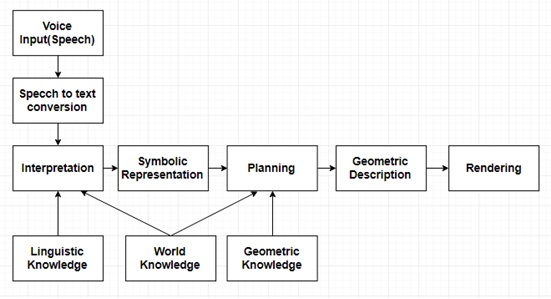
\includegraphics[width=350px,height=300px]{architecture.jpg}}
	\caption{Architecture design}
	\label{fig:architecture}
\end{figure}

\newpage

\subsection{System Interface Description}
\paragraph{}
The software is a desktop application and thus, will work on Windows OS. The user will simply need to install the software and it will be ready to use. All the libraries and database files will run in the background, potentially using cloud, therefore the user will only need to download and install the installer and main file.\\
The APIs and libraries used by the software are Speech to Text API, SpaCy library and 3D Warehouse database/dataset. All the components are back end products and therefore beyond users’ control and reach. The knowledge/information sets are also integrated with the APIs and libraries hence not concerning the user.
\section{User Interface Design}

\subsection{Screen Images}
\begin{figure}[htbp]
	\centering
		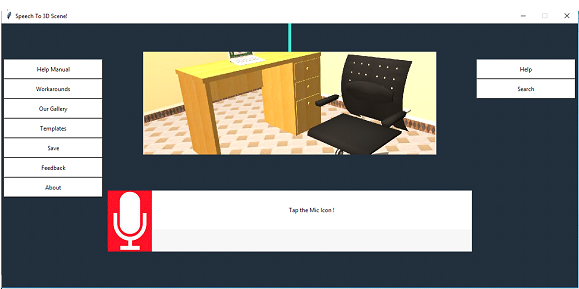
\includegraphics{ui2.png}
	\caption{User Interface}
	\label{fig:ui2}
\end{figure}
\newpage

\section{Design Document}
\subsection{Level 0 DFD}
\begin{figure}[htbp]
	\centering
		\frame{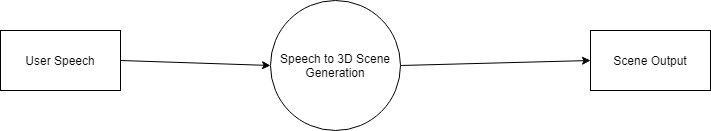
\includegraphics[width=390px]{dfd0.png}}
	\caption{DFD Level 0}
	\label{fig:dfd0}
\end{figure}

\subsection{Level 1 DFD}
\begin{figure}[htbp]
	\centering
		\frame{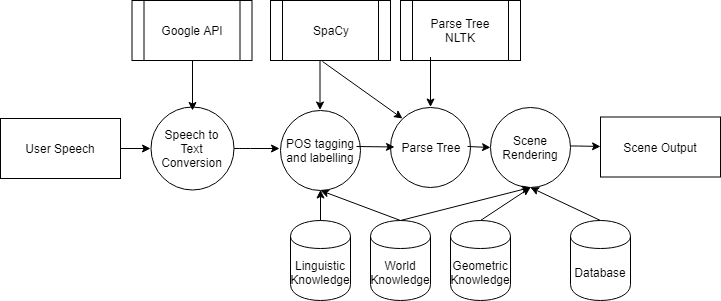
\includegraphics[width=380px,height=200px]{dfd1.png}}
	\caption{DFD Level 1}
	\label{fig:dfd1}
\end{figure}

\newpage

\subsection{Use Case Diagram}
\begin{figure}[htbp]
	\centering
		\frame{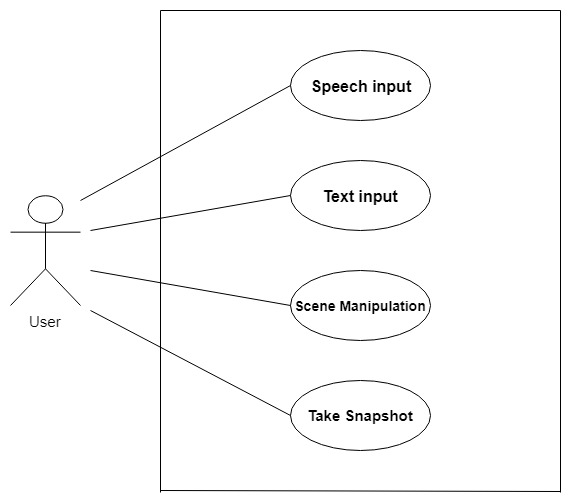
\includegraphics[width=390px]{Use_Case_Diagram.jpg}}
	\caption{Use Case Diagram}
	\label{fig:Use_Case_Diagram}
\end{figure}

\newpage

\subsection{Class Diagram}
\begin{figure}[htbp]
	\centering
		\frame{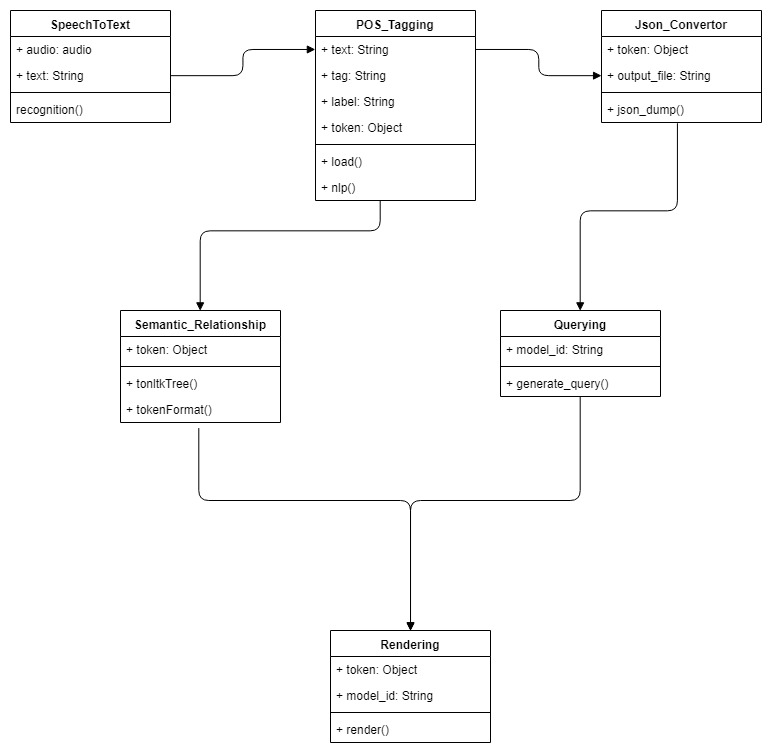
\includegraphics[width=390px]{Class_Diagram.jpg}}
	\caption{Class Diagram}
	\label{fig:Class_Diagram}
\end{figure}

\newpage

\subsection{Activity Diagram}
\begin{figure}[htbp]
	\centering
		\frame{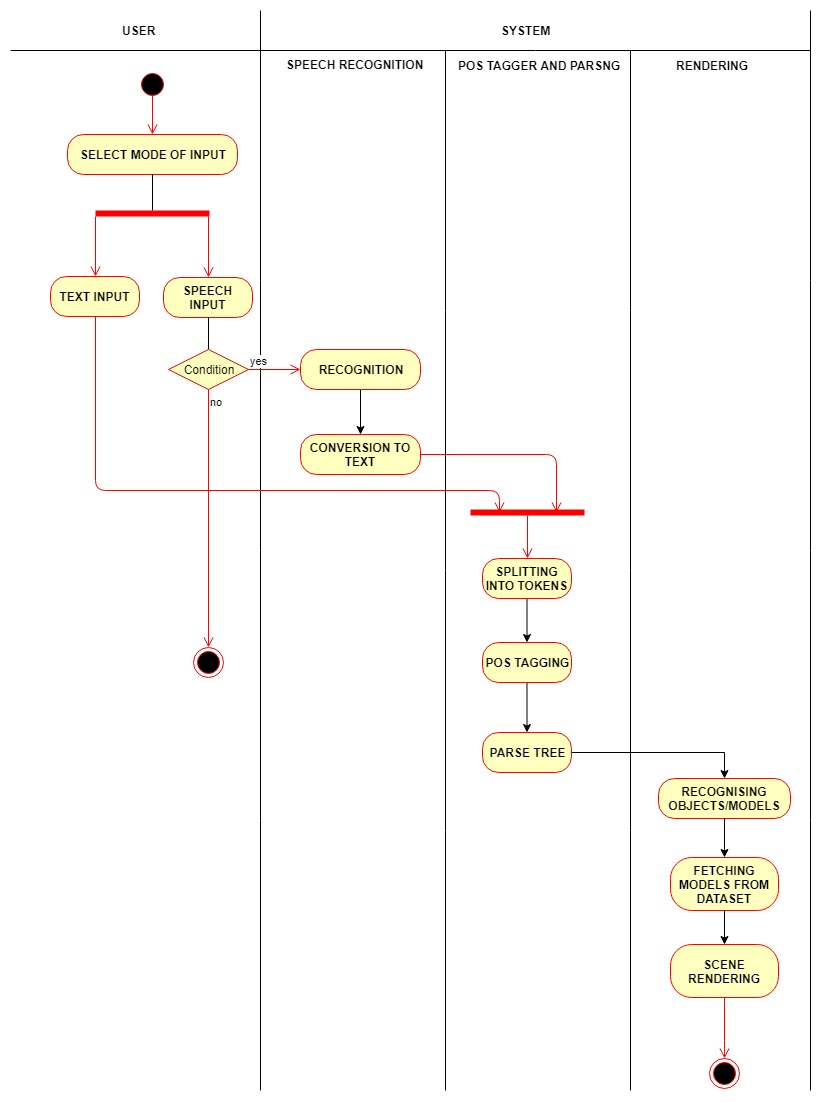
\includegraphics[width=390px,height=430px]{Activity_Diagram.jpg}}
	\caption{Activity Diagram}
	\label{fig:Activity_Diagram}
\end{figure}